% \input utf8-t1
\documentclass[10pt,titlepage,a4paper]{extarticle}

% ------ PACKAGES ------

\usepackage[czech]{babel}
\usepackage[utf8]{inputenc}
\usepackage{hyperref}
\usepackage{listings}
\usepackage{color}
\usepackage{xcolor}
\usepackage{newverbs}
\usepackage{todonotes}
\usepackage{graphicx}
\usepackage{float}
\usepackage{lipsum}
\usepackage{svg}
\usepackage{caption}
\usepackage{wrapfig}


% ------ CONFIGURATION ------

\colorlet{violet}{blue!80!red}
\colorlet{lightgray}{gray!5}

\colorlet{jsonnumber}{blue}
\colorlet{jsonpunct}{red}
\colorlet{jsondelim}{violet}

% default width of svg
\setsvg{width=.5\textwidth}
\graphicspath{{images/}}

% reset ref section names
\def\sectionautorefname{}
\def\subsectionautorefname{}
\def\subsubsectionautorefname{}

\renewcommand\lstlistlistingname{Seznam zdrojových kódů}
\renewcommand\lstlistingname{Zdrojový kód}



% ------ CUSTOM COMMANDS ------

% \ic for inline code
\makeatletter
\newcommand\ic[1][green]{%
    \@testopt{\@ic{#1}}{-#1}% Handle second optional argument
}
\def\@ic#1[#2]{%
    \Collectverb{\@@ic{#1}{#2}}%
}
\def\@@ic#1#2#3{%
    %\begingroup
    %\fboxrule=0.9\baselineskip
    %\fboxsep=...
    \fcolorbox{white}{lightgray}{\lstinline[basicstyle=\ttfamily\color{violet},breaklines=true]|#3|}%
    %\endgroup
}
\makeatother

% ref as <number of section> <title of section>
\newcommand*{\fullref}[1]{\hyperref[{#1}]{\autoref*{#1} \nameref*{#1}}}

\newenvironment{bottompar}{\par\vspace*{\fill}}{\clearpage}

% ------ LISTINGS SETUP ------

\lstset{
    language=Python,
    frameround=fttf,
    breaklines=true,
    keywordstyle=\color{violet!50!red}\ttfamily,
    basicstyle=\color{violet},
    numberstyle=\color{black},
    backgroundcolor=\color{white},
    frame=single,
    tabsize=4,
    breaklines=true,
    captionpos=t,
    xleftmargin=\fboxsep,
    xrightmargin=-\fboxsep,
    numberstyle=\scriptsize,
    numbersep=6pt,
    numbers=left,
}
\DeclareCaptionFormat{listing}{%
	\colorlet{currentcolor}{.}%
	{\color{violet}{\framebox[\textwidth+\fboxsep+\fboxsep+1pt]{\color{currentcolor}#1#2#3}}}%
}
\captionsetup[lstlisting]{format=listing, singlelinecheck=false}

\lstdefinelanguage{json}{
    basicstyle=\color{violet},
    numberstyle=\scriptsize,
    numbersep=8pt,
    numbers=left,
    breaklines=true,
    frame=single,
    %backgroundcolor=\color{background},
    literate=
     *{0}{{{\color{jsonnumber}0}}}{1}
      {1}{{{\color{jsonnumber}1}}}{1}
      {2}{{{\color{jsonnumber}2}}}{1}
      {3}{{{\color{jsonnumber}3}}}{1}
      {4}{{{\color{jsonnumber}4}}}{1}
      {5}{{{\color{jsonnumber}5}}}{1}
      {6}{{{\color{jsonnumber}6}}}{1}
      {7}{{{\color{jsonnumber}7}}}{1}
      {8}{{{\color{jsonnumber}8}}}{1}
      {9}{{{\color{jsonnumber}9}}}{1}
      {:}{{{\color{jsonpunct}{:}}}}{1}
      {,}{{{\color{jsonpunct}{,}}}}{1}
      {\{}{{{\color{jsondelim}{\{}}}}{1}
      {\}}{{{\color{jsondelim}{\}}}}}{1}
      {[}{{{\color{jsondelim}{[}}}}{1}
      {]}{{{\color{jsondelim}{]}}}}{1},
}

% ------ HYPERREF SETUP ------
\hypersetup{
	colorlinks,
	linkcolor={red!50!black},
	citecolor={blue!50!black},
	urlcolor={blue!80!black},
}

\begin{document}

\title{PYBOTS - hra pro programátory}
\author{Josef Kolář}
\date{\today}

\maketitle

\newpage
\section*{Prohlášení}
\thispagestyle{empty}
\todo{okopírovat prohlášení od SHN}
\clearpage

\begin{bottompar}
\section*{Poděkování}
\thispagestyle{empty}
\lipsum[1]
\todo{Poděkovat všem}
\clearpage
\end{bottompar}

\begin{abstract}
\todo{sepsat abstrakt}
\lipsum[2]
\end{abstract} 

\tableofcontents
\addcontentsline{toc}{section}{Obsah}

\newpage

\section{Teoretický úvod}

\subsection{Rozbor zadání}
\todo{scan zadání + rozbor jednotlivých bodů}
\subsection{Návrh architektury aplikace}

\subsubsection{Návrh interní struktury}

\textit{
	V této sekci se budu zabývat pouze teoretickým návrhem jednotlivých datových a řídící struktur. Popisu použitých algoritmů a jednotlivých implementačních rozhodnutí se budu věnovat v sekci \fullref{sec:implementation}.
}

O interní reprezentaci jedné instance hry se stará třída \ic|Game|, která je zodpovědná za striktní přístup klienta do mapy. Zpracovává jednotlivé herní akce klientů, kontroluje jejich validitu a aplikuje změny do mapy. \ic|Game| je sama schopna se vyexportovat do slovníku, který je následně převeden do formátu JSON a distribuován ke klientovi. Při herních akcích překládá výjimky vyvolané interně uloženou mapou na ty zvenku známé. V případě módu hry s tahy hlídá \ic|Game| pořadí jednotlivých botů.

Třída \ic|Game| interně využívá třídu \ic|Map| k uchování stavu hry. Třída \ic|Map| je v podstatě pouze zapouzdřený dvourozměrný kontejner reprezentující vlastní mapu. Je zodpovědná za validní přístup - tzn. mj. ošetřuje stavy pro nevalidní přístup mimo rozsah mapy.

Společným předkem pro všechny entity uložené v mapě je třída \ic|Field|. Jejím nejprimitivnějším potomkem je prázdné pole \ic|EmptyField|.

Existenci bota v mapě reprezentuje třída \ic|BotField|, která je zopovědná za udržení jeho prostorové orientace a umí se na místě otáčet. V případě, že se jedná o hru s bateriemi, je tato třída nahrazena třídou \ic|LaserBatteryBotField|, která se kromě orientace stará i o stav baterie. Ten je řízen pomocí metod \ic|LaserBatteryBotField.charge()| pro nabíjení, resp. \ic|drain()| pro vybíjení. Výjimka \ic|CriticalBatteryLevel| je vyvolána v případě, kdy by mělo dojít k vybití baterie pod nulovou úrove\v{n}.

Mezi další pomomky třídy \ic|Field| patří \ic|BlockField| reprezentující v mapě pole pevného bloku a \ic|TreasureField| zastupující poklad ve hře.

Třída, která kontroluje jednotlivé instance \ic-Game- v aplikaci se příznačně nazývá \ic|GameController|. Je zodpovědná delegování klientského požadavku na herní akci na odpovídající instanci hry. Zároveň zodpovídá za vytváření her, resp. na svém vstupu příjmá instanci potomka třídy \ic|BaseConfiguration|, kterou následně předá do singletonu třídy \ic|MapFactory|, která sestaví instanci mapy.

\ic|MapFactory| je třída zodpovědná za vygenerování mapy v závislosti na předané configuraci. Ze zadání plynou následující konfigurovatelné parametry:

\begin{center}
\begin{tabular}{llll}
český název & název parametru & vysvětlení & datový typ \\
\hline
šířka mapy & \ic|map_width| & počet bloků na šířku mapy & int \\
výška mapy & \ic|map_heigth| & počet bloků na výšku mapy & int \\
počet botů & \ic|bots| & maximální počet botů ve hře & int \\
počet bloků & \ic|blocks| & maximální počet bloků ve hře & int \\
počet pokladů & \ic|treasures| & počet pokladů ve hře & int \\
hra s tahy & \ic|rounded_game| & hra botů v pořadí & bool \\
hra s bateriemi & \ic|battery_game| & hra botů s bateriemi & bool \\
hra s lasery & \ic|laser_game| & hra botů s možností laseru & bool \\
\end{tabular}
\end{center}

\subsubsection{Návrh vnějšího rozhraní}
\todo{probrat URL, metody v závislosti na URL}
\subsection{Administrace}
\todo{změna konfigurace z formuláře, mazání her, náhled na hru}


\section{Interní implementace projektu}
\label{sec:implementation}

\subsection{Enumerace Orientation}

Tato enumerace dědící ze třídy \ic|IntEnum| z balíčku \ic|enum| zajištuje především sjednocení udávaných orientací v projektu, v některých případech označuje i směr. Je označena dekorátorem \ic|unique|, který zajištuje unikátnost jednotlivých hodnot v enumeraci. Tato enumerace obsahuje klíče \ic|NORTH|, \ic|EAST|, \ic|SOUTH| a \ic|WEST| s hodnotami v rozsahu od 1 do 4. Jako jednoduché utility jsou ve třídě metody (resp. vlastnosti díky dekorátoru \ic|@property|) \ic|is_horizontal| a \ic|is_vertical| ověřující horizontální, resp. vertikální směr. Výhoda v předkovi \ic|IntEnum|, resp. \ic|Enum| tkví v možnosti testovat shodnost pomocí operátoru rovnosti a konstruovat tyto objekty pomocí číselné hodnoty, viz následující ukázka.

\begin{lstlisting}[caption={Výhody třídy Enum}]
orientation_by_key = Orientation.NORTH
orientation_by_value = Orientation(0)

assert orientation_by_value == orientation_by_key
\end{lstlisting}

\subsection{Enumerace Action}

Enumerace \ic|Action| se v projektu používá jako jednoznačný identifikátor akce pro jednotlivé boty. Je stejně jako \ic|Orientation| odekorována pomocí \ic|@unique|, ale narozdíl od ní se nejedná o číselnou enumeraci, ale o enumeraci řetězců - pro snažší identifikaci v rámci požadavků na server.
Mezi její hodnoty patří \ic|STEP| pro pohyb robota, \ic|TURN_LEFT| a \ic|TURN_RIGHT| pro jeho otáčení, \ic|WAIT| pro čekání na místě (a nabití baterie) a \ic|LASER_BEAM| pro aktivaci laserového paprsku.

\subsection{Kontejnerová třída Map}

\ic|Map| je implementována jako dvourozměrná instance datového typu \ic|list|. Při inicializování objektu je ihned v konstruktoru (metoda \ic|__init__|) vytvořen dvourozměrný seznam - první rozměr pro výšku, druhý pro šířku. Oba tyto parametry jsou předány konstruktorem a je ověřena jejich nenulovost. Celý kontejner je naplněn instancemi třídy \ic|EmptyField|. Mezi další metody této třídy patří \ic|get_field_occurrences|, vracející seznam souřadnic, na kterých se nachází instance předáné třídy. Slouží k vyhledávání nad mapou, ale bohužel je její složitost vzhledem k implementaci $O(n^2)$. Metoda \ic|get_next_field| je určena k získávání vedlejší pole dle zadaných souřadnit a instance třídy \ic|Orientation|. V případě nemožnosti získat další pole ve směru na kraji mapy je vráceno \ic|None|. 

Níže uvedení příklad znázorňuje přetížené indexování instancí třídy \ic|Map| pomocí pozice uložené v vestavěném datovém typu \ic|tuple| (nebo jakýkoliv jiný objekt, který implementuje metodu \ic|__iter__|). Výsledkem je instance prázdného herního pole.

\begin{lstlisting}[caption={Přetížené indexování třídy Map}]
position = 3, 2
game_map = Map(width=10, height=10)

assert isinstance(
	game_map[position],
	EmptyField
)
\end{lstlisting}

\subsection{Třídy reprezentující herní bloky}

\subsubsection{Společný abstraktní předek Field}
\subsubsection{Prázdné pole EmptyField}
\subsubsection{Pole bloku BlockField}
\subsubsection{Pole pro poklad TreasureField}
\subsubsection{Pole pro boty BotField a LaserBatteryBotField}

\section{Použité technologie}

\subsection{Python}

\begin{wrapfigure}{R}{0.5\textwidth}
 \centering
 \includesvg[width=0.5\textwidth]{images/python-logo}
 \caption{Logo programovacího jazyka Python}
\end{wrapfigure}

Python je moderní interpretovaný programovací jazyk, který byl navržen v roce 1991 nizozemským programátorem Guido van Rossumem. Nabízí rozličná programovací paradigma: imperativní, procedurální, funkcionální nebo objektově orientované, které jsem ve své práci použil nejčastěji.

Python je vyvíjen jako open source projekt, jeho zdrojové kódy jsou tedy veřejné a je možné do nich přispět. Jeho výchozí implementace se nazývá \uv{CPython} dle jazyka C, ve kterém je implementována. Mezi další jeho alternativní implementace patří \uv{Jython} naprogramovaný v jazyce Java nebo \uv{IronPython} v prostředích .NET a Mono.

Jednou z velkých výhod Pythonu je jeho rozšířitelnost. Oficiální portál pro rozšiřující balíčky \href{https:\/\/pypi.python.org\/pypi}{PyPi} aktuálně nabízí okolo 74 tisíc knihoven. Kterýkoliv z těchto balíčků je možno pomocí nástroje pip nainstalovat a používat. Jednou z dalších možností, jak rozšířit jeho funkčnost, je naprogramovat si vlastní rozšíření v jazyce C.

Python je aktuálně vyvíjen ve dvou hlavních větvích; větvi Pythonu verze 2 a verze 3. Motivace pro vydání verze 3 byla především ve sjednocení práce s řetězci (Python verze 2 rozlišoval řetězce ASCII znaků a řetězce Unicode znaků), celočíselného dělení a některých syntaktických vylepšení jazyka. Poslední vydaná verze Pythonu je 3.5 a její hlavní výhodou je přidání podpory pro asynchronní volání funkcí a podpory pro typovost parametrů a návratových hodnot funkcí a metod.

\subsubsection{Jednotkové testování}

Jednotkové automatické testování je jeden z způsobů, jak vývojáři ulehčit úpravu, vytváření i mazání částí zdrojových kódů. Jednotka testu je v množina asercí (předpokladů), které kontrolují vývojářem vytvořené modelové situace nad zdrojovým kódem programu. Automatické testování je poté automatické spouštění testů např. po změně zdrojového kódu a určení, zda testy prošly korektně (aserce všech testů jsou pravdivé). Samotný test je však psán samotným vývojářem, což při testování může vytvářet klamný dojem \uv{bezchybnosti} zdrojového kódu projektu, protože vývojář jakožto člověk, je bytost chybující a samotný kód testů může být napsat chybně a aserce jsou v tu chvíli bezpředmětné, protože jsou např. vždy pravdivé a znehodnocují tím korektnost  a správnost testů projektu.

Níže je uveden příklad třídy k testování. Třída \ic-MathOperations- je určena k základním matematickým operacím, pro názornost pro sčítání a dělení. 
\begin{lstlisting}[caption={Příklad třídy MathOperations k testování}]
class MathOperations(object):
	@staticmethod
	def add(a, b):
		return a + b

	@staticmethod
	def divide(a, b):
		return a / b
\end{lstlisting}

\begin{sloppypar}
	Pomocí volání \ic|MathOperations.add(40, 2)| získáme \ic|42|, resp. při \ic|MathOperations.divide(36, 6)| je výsledkem \ic|6|. Ve své práci používám balíček pro testování \ic|unittest| dodávaný přímo s programovacím jazykem Python. Jako hlavní nástroj pro jednotkové testování nabízí tento balíček třídu \ic|TestCase|, která obsahuje celou řadu metod pro testování asercí (\ic|assertEqual|, \ic|assertTrue|, \ic|assertEqual|, \ic|assertIn|, \ic|assertIs| nebo i komplexnější jako \ic|assertDictEqual|, \ic|assertRegex| nebo \ic|assertDictContainsSubset|) a potomky této třídy je potom možno automaticky spouštět a vyhodnocovat. Tyto předpoklady tedy zapíšeme jako metody do obalující třídy:
\end{sloppypar}

\begin{lstlisting}[caption={Základní TestCase pro třídu MathOperations}]
class TestMathOperations(TestCase):
	def test_add(self):
		self.assertEqual(
			MathOperations.add(40, 2),
			42
		)

	def test_div(self):
		self.assertEqual(
			MathOperations.div(36, 6),
			6
		)
\end{lstlisting}

V případě spuštění a úspěšného otestování této třídy by byl výstup tento:
\begin{lstlisting}[language=bash, caption={Ukázka výstupu ze spuštění testů}]
test_add (TestMathOperations) ... ok
test_div (TestMathOperations) ... ok

------------------------------------
Ran 2 tests in 38ms

OK
\end{lstlisting}


\textit{
	Ve svém projektu používám vlastní poděděnou třídu
}
\todo{opravit kurzívu společně s inline kódem}
\ic|TestCase|
\textit{
, protože pro každé pokročilejší testování pohledů frameworku Flask je nutné mít správně nakonfigurovaný objekt pro \uv{vnější} přístup ke serveru, a také kvůli zobecnění některých častých operací v mých testech - detaily ohledně testů jsou v sekci \fullref{sec:implementation}.
}


Poté ale může dojít k následující změně zdrojového k\'{o}du - vznikne požadavek na metodu \ic|MathOperations.add|, a to konkrétně na zvýšení počtu parametrů na tři. Ne ve všech případech se ovšem bude volat tato metoda i se třetím parametrem, musí být tedy zajištěna \textbf{zpětná kompatibilita}.
\begin{lstlisting}[caption={Vylepšená implementace metoda MathOperations.add}]
@staticmethod
def add(a, b, c=0):
	return a + b + c
\end{lstlisting}
Do metody testující sčítání je tedy nutné přidat aserci i pro tři parametry:
\begin{lstlisting}[caption={Testovací metody pro upravenou implementaci MathOperations.add}]
def test_add(self):
	self.assertEqual(
		MathOperations.add(40, 2),
		42
	)
	self.assertEqual(
		MathOperations.add(10, 7, 3),
		20
	)
\end{lstlisting}
Tímto testem máme potvrzenou korektní jak pro dvouparametrické volání, tak pro \uv{nové} tříparametrické volání. Podstata úprava zdrojového kódu tkví v zachování předchozích asercí - je tak zajištěna zpětná kompatibilita. Jako další požadavek na metodu \ic|MathOperations.add| může typicky přijít přidání dalšího parametru, kdy je vhodné vzhledem k aktuální implementaci metody \ic|add| tuto metodu přeimplementovat následovně:
\begin{lstlisting}[caption={Finální implementace metody MathOperations.add}]
@staticmethod
def add(*values):
	return sum(values)
\end{lstlisting}
\textit{
  Zápis \\ic|*values| je velmi specifický pro jazyk Python. 
}
A ke testovacím asercím přidat i jednu komplexnější obsahující volání s vytším počtem parametrů:
\begin{lstlisting}[caption={Finální test pro metody MathOperations.add}]
def test_add(self):
	...
	values = tuple(randint(0, 100) for _ in range(10))
	self.assertEqual(
		MathOperations.add(*values),
		sum(values)
	)
\end{lstlisting}
\subsection{Flask}

% \begin{figure}[H]
%  \centering
%  \includesvg[width=.3\textwidth]{images/flask-logo}
%  \caption{Logo webového frameworku Flask}
% \end{figure}

\begin{wrapfigure}{R}{\textwidth/3}
    \centering
    
\includegraphics[width=\textwidth/3]{images/flask-logo}
    \caption{Logo webového frameworku Flask}
\end{wrapfigure}

Flask je webový framework implementovaný v jazyce Python. Mezi jeho přednosti patří vestavěný vývojářský server, plná podpora pro unit testování a kvalitní dokumentace. Vzhledem k jeho variabilitě a v základu tenké architektuře bylo nutné přidat abstraktní vrstvy pro samotné zpracování herních akcích a podobně.

Vzhledem k tomu, že je framework téměř stoprocentně pokryt testy, lze jednoduše usuzovat z těchto testů o funkčnostech frameworku a také je velmi snadné psát vlastní testy na kteroukoliv komponentu aplikace.

\subsection{HTTP}

HTTP (HyperText Transfer Protocol) je standardizovaný internetový protokol pro výměnu HTML kódu. Jeho první koncept vznikl v roce 1991 jako veze 0.9, o pět let později byla uvedena verze 1.1 a verze 1.1, která je používaná dodnes byla uvedena v červu roku 1999. V dnešní době je používán nejen k výměně HTML kódu, ale jeho rozšíření MIME \footnote{Multipurpose Internet Mail Extensions} poskytuje možnost přenosu souborů jakéhokoliv typu. Samotný HTTP nezajištuje zabezpečení ani integritu dat. Nadstavbu nad HTTP tvoří HTTPS, jehož komunikace je šifrována pomocí SSL nebo TLS.

HTTP pracuje na principu request-response (požadavek-odpověd). HTTP požadavek ve formě plaintextu je vyslán ze klientského zařízení, ten je serverem zpracován a nazpět jsou odeslány tzv. hlavičky odpovědi a poté i samotné její tělo. Vzhledem k tomu, že každý další následující dotaz klienta na server bude nezávislý na těch předchozích, je nutno označit tento protokol za bezstavový. Nelze tedy uchovávat stav komunikace a jednotlivé požadavky nemají mezi sebou souvislost. Tato vlastnost může být částečně potlačena použitím HTTP cookies, které jsou schopny téměř jednoznačně identifikovat klientské zařízení na serveru.

\subsection{JSON}

JavaScript Object Notation je datový formát pro přenos dat nezávislý na platformě. Oproti jeho hlavnímu konkurentu XML je datově úspornější, avšak je nevhodný k přenosu binárních informací. JSON je schopen kódovat a následně dekódovat tyto datové typy:

\begin{itemize}
    \item
    \textbf{integer} - celočíselné hodnoty jako 6, -3 nebo 0.

    \item
    \textbf{float} - desetinná čísla jako 6.6, -3.5 nebo 0.9.

    \item
    \textbf{string} - řetězec znaků, např. "bar".

    \item
    \textbf{boolean} - pravdivostní hodnoty \textit{true} a \textit{false}.

    \item
    \textbf{array} - standardní netypový seznam, např. [6, 3.5, "foo"].

    \item
    \textbf{object} - seznam prvků ve struktuře \textit{klíč} - \textit{hodnota}, např. \{"foo": 6, "bar": [1, 10, 100]\}.
\end{itemize}

\begin{figure}[H]
 \centering
 \includesvg{images/json-logo}
 \caption{Logo datového formátu JSON}
\end{figure}

Příklad pokročilé struktury tohoto formátu (jedná se o upravenou verzi JSON exportu z PYBOTS):

\begin{lstlisting}[language=json,caption={Ukázka datového formátu JSON}]
 {"map": [
    [
      1,
      {
        "field": 2,
        "orientation": 0,
        "your_bot": true
      }
    ],
    [
      0,
      3
    ]
  ], "map_resolutions": "2x2"
}
\end{lstlisting}

\section{Použité metatechnologie}

\subsection{Git}

\begin{wrapfigure}{R}{0.5\textwidth}
 \centering
 \includesvg[width=0.5\textwidth]{images/git-logo}
 \caption{Logo verzovacího systému Git}
\end{wrapfigure}

Git je distribuovaný systém správy verzí, původně určený pro vývoj jádra Linuxu. Jako jeho autor je označován Linus Torvalds, jeho vznik se datuje kolem 2005 a v roce 2016 je nadále aktivně vyvíjen; jeho poslední verze nese označení 2.7.3 a byla vydána 10. března 2016. Nejčastěji slouží k verzování zdrojového kódu - vytváří historii pro každou část spravovaného repozitáře. Repozitář je v tomto systému základní nejvyšší jednotka pro správu zdrojového kódu, zapouzdřuje jednotlivé vývojové větvě, ve kterých může probíhat vývoj od jednotlivých vývojářů zcela odděleně. Git je oproti jiným verzovacím nástrojům velmi silný v následném spojování těchto větví - v případě nekonfliktních změn je toto spojení schopen provést zcela sám.

Git je plně ovladatelný z příkazové řádky, avšak existuje velké množství jeho grafických nadstaveb, například jednoduchý \href{http://git-cola.github.io/}{git-cola} nebo omnoho komplexnější \href{https://www.sourcetreeapp.com/}{SourceTree}.

\begin{figure}[H]
 \centering
 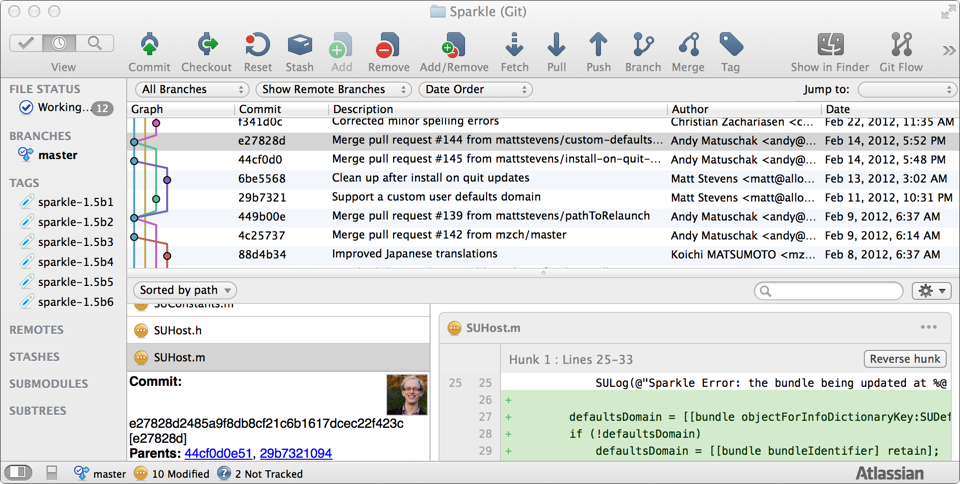
\includegraphics[width=\textwidth]{images/source-tree-screenshot}
 \caption{Screenshot z programu SourceTree}
\end{figure}

\begin{figure}[H]
 \centering
 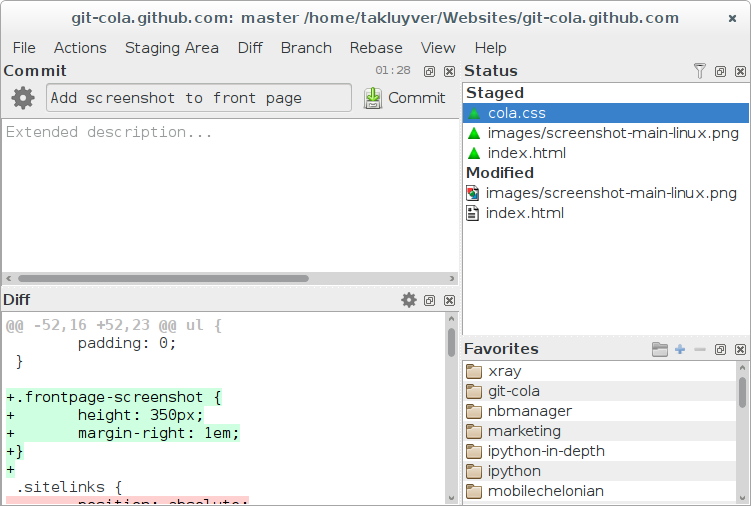
\includegraphics[width=\textwidth]{images/git-cola-screenshot}
 \caption{Screenshot z programu git-cola}
\end{figure}

\subsection{Github}

Github je webová služba poskytující podporu pro hostování git repozitářů. Pro veřejné repozitáře je tato služba zcela zdarma, pro soukromé repozitáře je zpoplatněna. Kromě hostování nabízí i širokou škálu služeb týkajících se zdrojového kódu, jako například komentování zdrojového k\'{o}du, komentování jeho změn, systém úkolů, soukromých zpráv mezi vývojáři nebo možnost zařazení repozitáře mezi oblíbené. Github spustili v roce 2008 Tom Preston-Werner, Chris Wanstrath a PJ Hyett.

\begin{figure}[H]
 \centering
 \includesvg{images/github-logo}
 \caption{Logo systému pro správu git repozitářů GitHub}
\end{figure}

\subsection{Travis CI}

\begin{figure}[H]
 \centering
 \includesvg{images/travis-logo}
 \caption{Logo automatického buildovacího nástroje Travis CI}
\end{figure}

\subsection{Pycharm}

\begin{figure}[H]
 \centering
 \includesvg{images/pycharm-logo}
 \caption{Logo vývojového nástroje Pycharm}
\end{figure}

\section{Závěr}

Podařilo se mi naprogramovat herní server v plném rozsahu zadání.
\todo{Zhodnotit a sepsat, jak je vše super}

\subsection{Možná budoucí vylepšení}

\begin{itemize}
 \item pro bezpečnější použití by bylo vhodné znovu navrhnout a vylepšit systém autorizace k přístupu k ovládání bota - \ic|bot_id| jakožto soukromý klíč přenášený po HTTP protokolu není nejbezpečnější metoda
 \item přidat herní log, ze kterého bude možné zrekonstruovat celý průběh hry od vygenerování až po vítězství jednoho z botů  
 \item do samotné hry je poměrně snadné přidat herní prvky, takže není problém přidat bonusové herní bloky, teleporty bloků, systém min nebo obranná elektromagnetická pole
\end{itemize}


\newpage

\listoffigures
\addcontentsline{toc}{section}{Seznam obrázků}

\lstlistoflistings
\addcontentsline{toc}{section}{Seznam zdrojových kódů}

\end{document}
